\documentclass[a4paper,12pt]{article}
\usepackage{polski}
\usepackage[utf8]{inputenc}
\usepackage{graphicx}
\author{Marcin Fabrykowski}
\title{Bezpieczeństwo w sieci. Ochrona sieciowa. Lab 04}
\begin{document}
\maketitle
\newpage
\part{Wstęp}
\section{Co to jest iptables?}
Iptables jest programem pozwalającym na konfiguracje wbudowanego w jądro linuxa filtra pakietów. Iptables służy również do konfigurowania NAT-u.
\subsection{Co to jest NAT?}
Network Address Translation - system translacji adresów sieciowych. Wykorzystywany tam, gdzie nie każdy klient ma swój adres publiczny, a jedynie taki posiada. Pozwala on na komunikację komputerom za natem ze światem. Klienci za NATem posiadają swoje adresy prywatne, niewidoczne dla świata.\\
NAT dzielimy na dwie grupy:
\begin{enumerate}
\item SNAT - Source NAT. Wykorzystywany, gdy chcemy żeby klient mógł połączyć się ze światem, a nie tylko z siecią lokalna. Jest to chyba najczęściej wykorzystywany NAT.\\
Zasada działania: Kiedy klient próbuje wysłać pakiet w świat, wysyła on go z adresem docelowym "światowym" do routera. Tam zostaje zamieniony adres źródłowy z prywatnego klienta, na publiczny routera.
Dzieje się tak dlatego, żeby host docelowy, chcąc odpowiedzieć, mógł skierować odpowiedź do routera który jest widoczny ze świata, a ten dopiero przekaże odpowiedź do klienta. 
\item DNAT - Destination NAT. Rzadziej wykorzystywany. Realizuje on sytuację odwrotną. Gdy jakaś zewnętrzna stacją chce się podłączyć do komputera za NATem, nie ma takiej możliwości bez wykorzystania DNATu. Gdy przychodzi pakiet ze świata na router i zostanie on sklasyfikowany jako pakiet przeznaczony do wnętrza sieci, zostaje podmieniony adres docelowy (routera) na prywatny adres maszyny w sieci i pakiet jest wpuszczany.
\end{enumerate}
\section{Po co jest iptables?}
Iptables pozwala na filtrowanie pakietów przychodzących, wychodzących i przechodzących przez filtrowaną maszynę. Pozwala także na modyfikowanie tych pakietów jak i ich logowanie.
\section{Jak działa iptables?}
Iptables analizuje każdy pakiet który przychodzi do niego. Przepuszczany jest on przez serię tablic. Schemat przejścia pakietu po tablicach, pokazuje rys. \ref{fig:iptables_tablice}.
\begin{figure}
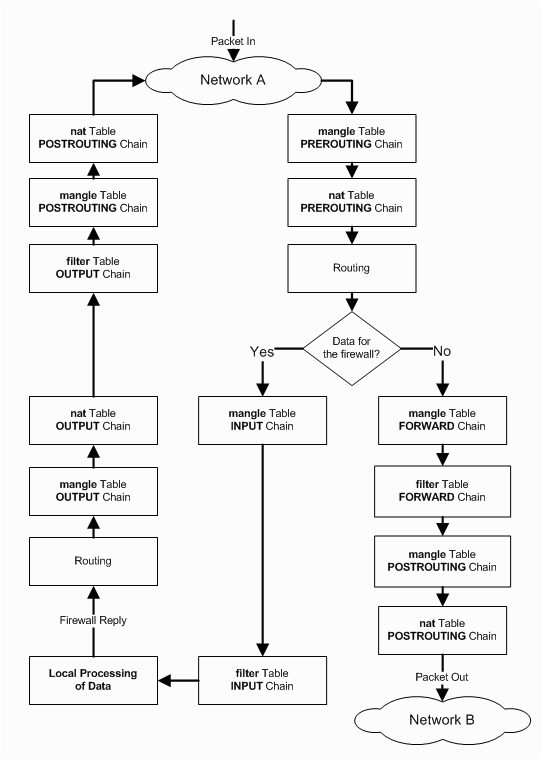
\includegraphics[scale=0.8]{iptables.png}
\caption{Schemat przejścia pakietu po tablicach w iptables}
\label{fig:iptables_tablice}
\end{figure}
\section{Dla kogo jest iptables?}
\begin{enumerate}
\item Z poziomu zwykłego użytkownika, pozwala on zabezpieczyć nasz komputer przed niepożądanymi połączeniami przychodzącymi jak i wychodzącymi.
\item Z punktu widzenia administratora sieci, pozwala na ochronę serwera przed złym światem, jak również na logowanie i filtrowanie ruchu z i do sieci.
\end{enumerate}
\section{Co potrafi iptables?}
\subsection{Rozpoznawanie pakietów}
Iptables potrafi dopasować pakiety wedle wielu różnych kryteriów, m.in.:
\begin{itemize}
\item protoków
\item adres źródłowy
\item adres docelowy
\item interfejs wejściowy
\item interfejs wyjściowy
\item port źródłowy
\item port docelowy
\item flagi TCP
\item typ ICMP
\item mark
\item liczbie pakietów na jednostkę czasu
\item MAC adres
\item TTL
\item dzień,godzina
\end{itemize}
i wiele innych kryteriów pozwalających dokładnie określić, który pakiet należy zaakceptować a który odrzucić
\subsection{Decydowanie o pakiecie}
Po dopasowaniu pakietu, należy zdecydować, co z takim pakietem zrobić. Najpopularniejszymi akcjami jakie można zrobić z pakietami są:
\begin{itemize}
\item zaakceptować
\item odrzucić
\item sklasyfikować
\item DNAT
\item SNAT
\item zalogować
\item zmienić ttl
\end{itemize}
oraz wiele innych
\subsection{Sekwencje wykonywania}
Iptables pozwala na bardziej przejrzyste budowanie firewalla poprzez tworzenie łańcuchów z własnymi sekwencjami akcji.
\end{document}
